\chapter{Dimensionality Reduction} 
\label{chapter-linear} 

As explained in section \ref{intro-framework}, our basis for comparison is the neural manifold, which is a lower-dimensional representation of the original neural output. This requires the use of an appropriate dimensionality reduction method\footnote{Linear dimensionality reduction methods work well when the data lie near a linear subspace of high-dimensional space. They suffice for the purpose of the project thus far, but when the data lie near a nonlinear manifold , a nonlinear dimensionality reduction method might be more suitable \cite{fefferman_testing_2016}. Therefore, we also introduce the nonlinear dimensionality reduction technique of diffusion map in Appendix \ref{appendix-diffmap}.}. In this thesis, we focus on the linear dimensionality reduction method, tensor CANDECOMP/PARAFAC (CP) decomposition, a higher-order generalization of Principal Component Analysis (PCA)\footnote{In this chapter we assume familiarity with PCA, but interested reader could refer to Appendix \ref{appendix-pca} for notes on PCA.}. This higher-order generalization is necessary because the neural output has three dimensions, namely neurons, stimuli, and time steps (which will be further explained in Chapter \ref{chapter-biological}). 

\section{Tensor CP decomposition}
\begin{defn}[Tensor]
    An $N$-way \underline{tensor} is defined as an element of the tensor product of $N$ vector spaces. A $1$-way tensor is a vector. A $2$-way tensor is a matrix.
    \end{defn}

\begin{defn}[Tensor norm]
The \underline{norm of tensor} $\mathcal{X} \in \RR^{I_1 \times I_2\times\cdots I_N}$ is
\begin{align}
    \norm{\mathcal{X}} = \sqrt{\sum_{i_1 = 1}^{I_1}\sum_{i_2 = 1}^{I_2}\cdots \sum_{i_N = 1}^{I_N} x_{i_1 i_2 \dots i_N}^2 }.
\end{align}
\end{defn}
\begin{defn}[Rank-one tensor]
An $N$-way tensor $\mathcal{X} \in \RR^{I_1 \times I_2\times\cdots I_N}$ is \underline{rank-one} if it can be written as the outer product of $N$ vectors, that is,
\begin{align}
    \mathcal{X} = \aaa^{(1)}\circ \aaa^{(2)} \circ \cdots \circ \aaa^{(N)}
\end{align}
\end{defn}

Analogous to PCA, tensor CP decomposition aims to approximate the original tensor by a sum of rank-one tensors, each of which can then be written as the outer product of $N$ vectors. Given a $3$-way tensor $\mathcal{X} \in \RR^{I\times J\times K}$, the tensor CP decomposition model is formulated as
\begin{align}
    \mathcal{X} \approx [\![ \mathbf{A}, \mathbf{B}, \mathbf{C} ]\!] = \sum_{r=1}^R \aaa_r \circ \bbb_r \circ \ccc_r,
\end{align}
where $R$ is the rank of the tensor, i.e., the minimal number of rank-1 tensors necessary to represent the tensor. $a_r \in \RR^I, b_r \in \RR^J, c_r \in \RR^K$ for $r = 1,\dots, R.$ Determining the rank $R$ of a specific given tensor is difficult; in fact, the problem is NP-hard. Thus, typically the goal is to find the low-rank approximation of the true rank, i.e., $R$ as an approximation of the true rank $M$ and $R < M$.

% The element-wise formulation analogous to \ref{pca} is 
% \begin{align}
%     x_{i j k} \approx \sum_{r=1}^R a_{i r} b_{j r} c_{k r}
% \end{align}
% for $i = 1,\dots, I, j = 1,\dots, J, k = 1,\dots,K.$

With tensor CP decomposition, we obtain the tensor factors which are analogous to the principle components in PCA. These neural factors can then be used as lower-dimensional representation of the tensor data. This can be illustrated with the diagram below. These neural factors can be used as lower-dimensional representation of the tensor data.
\begin{figure}[H]
    \centering
        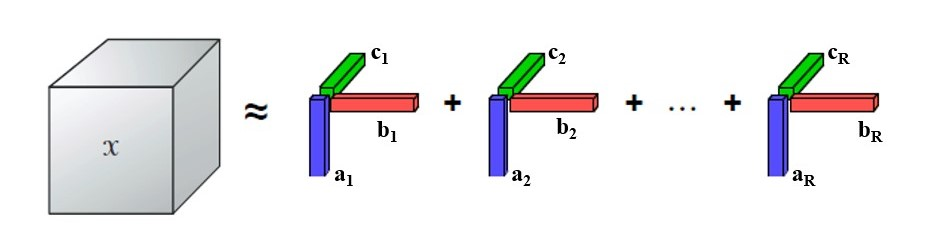
\includegraphics[width=0.7\textwidth]{figures/linear/tca.jpg}
        \caption{Illustration for tensor CP decomposition. (Adapted from \cite{williams_unsupervised_2018})}
    \end{figure} 

% The alternating least squares (ALS) method in \cite{kolda_tensor_2009} is one of the most common algorithms to compute a tensor CP decomposition with $R$ components. The steps of the ALS are summarized as follows: 
% \begin{enumerate}
%     \item fix  $\mathbf{B}$ and  $\mathbf{C}$ to solve for $\mathbf{A}$: 
%      \begin{equation}
%       \min_{\mathbf{A}} \sum_{i j k}\left(x_{i j k} - \sum_l a_{i l} b_{j l} c_{k l}\right)^2
%      \end{equation}
%     \item fix $\mathbf{A}$ and  $\mathbf{C}$ to solve for  $\mathbf{B}$:
%   \begin{align}
%       \min_{\mathbf{B}} \sum_{i j k}\left(x_{i j k} - \sum_l a_{i l}  b_{j l} c_{k l}\right)^2
%      \end{align}
%  \item fix $\mathbf{A}$ and  $\mathbf{B}$ to solve for $\mathbf{C}$: 
%  \begin{align}
%       \min_{\mathbf{C}} \sum_{i j k}\left(x_{i j k} - \sum_l a_{i l}  b_{j l} c_{k l}\right)^2
%      \end{align}
% \end{enumerate} 
% and repeat the above steps until some convergence criterion is satisfied. 

In selecting the optimization algorithm, we experimented with different optimization methods using the the generalized CP decomposition framework described in \cite{hong_generalized_2020}. In the end, gradient-based direct optimization approach (OPT) \cite{direct-opt}  was shown to give higher accuracy when the number of factors chosen is larger than the true rank (``overfactoring”). This could help inform us the number of factors to choose. 

Additionally, when the data has a non-negative constraint, Non-negative Tensor Factorization (NTF) is used. In NTF,
by adding the non-negative constraint, the original optimaization problem becomes:

 \begin{mini}|l|
  {\mathbf{A},\mathbf{B},\mathbf{C}}{\|\mathcal{X}- [\![ \mathbf{A}, \mathbf{B}, \mathbf{C} ]\!] \|_F^2}{}{}
  \addConstraint{\mathbf{A}, \mathbf{B}, \mathbf{C} \geq 0.}
 \end{mini}
Henceforth we will refer to the chosen linear dimensionality reduction method (tensor CP decomposition using direct optimization with non-negative constraint) as Non-negative Tensor Factorization (NTF).


